\chapter{Introduction}
\label{chap:theory}

\section{The Standard Model of Particle Physics}
\label{sec:theSM}

The \ac{SM} of fundamental interactions is the theory
which describes the electromagnetic, weak and strong nuclear interactions, often
represented as a collection of the elementary particles predicted by the theory.
The SM has successfully described data from a wide range of experiments, and in the 
years prior to the LHC, all of the predicted elementary particles were verified 
except for one: the Higgs boson.

\subsection{Particles and Forces} 

The \ac{SM} is a renormalisable quantum field theory, in which the constituents of
matter are represented as spin-$\frac{1}{2}$ fermions which interact with
forces mediated by spin-1 bosons. These interactions are described by a
Lagrangian which is invariant under $SU(3)_{C} \times SU(2)_{L} \times U(1)_{Y}$
symmetries. The $SU(3)_{C}$ part describes the strong interaction, mediated by
particles which carry colour charge (C). In these interactions, described by the
theory of \ac{QCD}\cite{}, the force mediators are massless gluons
and the coloured fermions are the quarks. The remaining fundamental fermions,
the leptons, do not carry colour charge and hence do not interact via the strong
force. Both the leptons and quarks participate in electroweak interactions,
which are governed by the $SU(2)_{L} \times U(1)_{Y}$ symmetry.

The electroweak symmetry describes the unified electromagnetic and weak
interactions\cite{}, and was one of the major achievements of the twentieth
century in the \ac{SM}. In electroweak theory the quantum numbers of interest are
weak isospin $t_{1,2,3}$ and hypercharge $y$. These are related to the
electric charge Q as: 

\begin{equation}
Q = t_{3} + \frac{y}{2}
\end{equation}

The gauge fields associated with these quantum numbers are the three weak isospin fields,
$W_{\mu}^{i}$, $i = 1,2,3$, and the hypercharge field $B_{\mu}$. The weak
isospin fields act on doublets: 

\begin{equation}
\begin{pmatrix} u_{i} \\ d_{i} \end{pmatrix}_{L} ,   
\begin{pmatrix} \nu_{i} \\ {l_{i}} \end{pmatrix}_{L}
\end{equation}

where $u_{i}$ are the up-type quarks ($u,c,t$), $d_{i}$ are the down-type quarks
($d,s,b$), $l_{i}$ are the charged leptons ($e,\mu,\tau$) and $\nu_{i}$ are the
corresponding neutrinos ($\nu_{e},\nu_{\mu},\nu_{\tau}$). The index $i$ indicates first, second or third
generation fermions. The subscript $L$ indicates that the doublets correspond to
the left handed projection of the fermions. The weak force only interacts with
left handed fermions, and as such is maximally parity violating. The right handed projections
transform as singlet states, which are invariant under $SU(2)_{L}$.

The physical $\gamma, Z$ and $W$ bosons result from mixing between the gauge
fields:

\begin{equation}
\begin{pmatrix} A_{\mu} \\ Z_{\mu}^{0} \end{pmatrix} = 
\begin{pmatrix} \cos{\theta_{W}} & \sin{\theta_{W}} \\ -\sin{\theta_{W}} &
\cos{\theta_{W}} \end{pmatrix} . 
\begin{pmatrix} B_{\mu} \\ W_{\mu}^{3} \end{pmatrix}
\end{equation}

where $A_{mu}$ is the photon field and $\theta_{W}$ is the weak mixing angle,
which can be related to the couplings of the weak neutral ($g$) and electromagnetic
interactions ($g'$) as $\theta_{W}=\tan^{-1}{\frac{g'}{g}}$. 

No mass terms. Need to add either lagrangian to prove this or find a hand wavey
way using the doublets and the interaction terms. Then we move on to EWSB,
having motivated it.

\cite{GlashowPartialSymmetries,WeinbergModelOfLeptons,SalamNobelSymposium}.

\subsection{The Higgs Mechanism in the \ac{SM}}
\label{sec:SMHiggs}


\begin{figure}[htbp]
   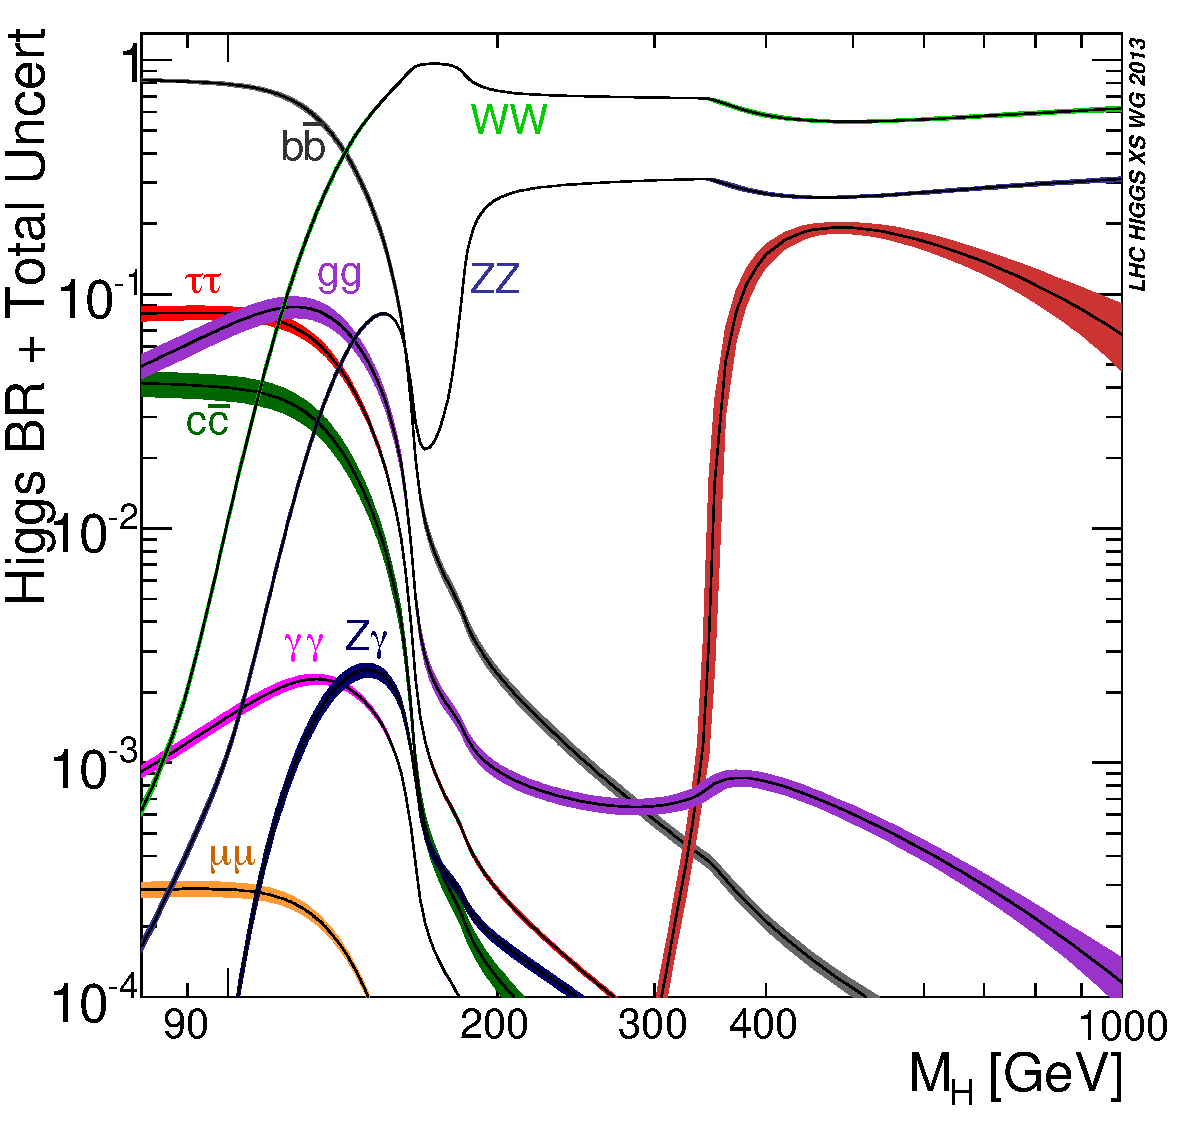
\includegraphics[width=0.5\textwidth]{plots/theory/Higgs_BR.pdf}
\caption{Higgs boson branching ratios in the \ac{SM}\cite{}.}
\label{fig:SMHiggsBRs}
\end{figure}


\subsection{Motivation for theories beyond the \ac{SM}}

Despite its successes, the \ac{SM} is known to have some shortcomings. One concerns
the calculations of the Higgs Boson mass, and is known as the Hierarchy problem. 

\section{Theories beyond the SM}
\label{sec:BSM}

\subsection{The Higgs sector in the MSSM}
\label{sec:mssmhiggs}

\section{Previous Searches for a Neutral Higgs boson}
\label{sec:previoussearches}

\subsection{MSSM Models incorporating the LHC Higgs}
\label{sec:mssmbenchmarks}

With the discovery of a 125$~\GeV$ Higgs-like particle at the LHC, the number of
possible MSSM scenarios is reduced to those which can incorporate this boson
with its measured properties. This section details some possible MSSM scenarios
which can incorporate this 125$~\GeV$ boson, whilst also exhibiting interesting
phenomenology motivated by experimental measurements. In particular the
scenarios must fulfil the condition $m_{\PH} = 125 \pm 3 \GeV$ over a wide range
of parameter space, and satisfy the boundaries set by previous searches at LEP,
the Tevatron and the LHC. The $3~\GeV$ uncertainty on the Higgs mass is
dominated by theoretical uncertainties in the MSSM models. All of the scenarios 
considered are defined without allowing CP violation. The scenarios follow those
described in~\cite{MSSMScenarios}, with some small modifications. More detail
can be found in~\cite{HIG-14-021}. 

As described previously, at tree level the masses of the five Higgs bosons are
defined by $m_{\PA}$ and $\tan\beta$. These masses are adjusted via radiative
corrections, necessary to produce a Higgs with mass consistent with $125~\GeV$.
The parameters of interest in these radiative corrections are as follows:

\begin{itemize}
\item The mass of the top quark, $m_{\Pqt}$.
\item The mass of the bottom quark, $m_{\Pqb}$.
\item The mass of the 3rd generation squarks: stops and sbottoms, given by
$M_{\text{SUSY}}$.
\item The higgsino mass parameter, $\mu$.
\item The mass of the 3rd generation sleptons: the staus, given by
$M_{\PSlepton_{3}}$.
\item The $U(1)$ gaugino mass parameter, $M_{1}$.
\item The $SU(2)$ gaugino mass parameter, $M_{2}$.
\item The trilinear couplings of the stops, sbottoms and staus, $A_{\Pqt}$,
$A_{\Pqb}$ and $A_{\Pgt}$.
\item The mixing parameters of the stops, sbottoms and staus, $X_{\Pqt}$,
$X_{\Pqb}$ and $X_{\Pgt}$.
\end{itemize}

The dependence on these parameters can be reduced by exploiting relations
between them. For most scenarios, $M_{1}$ and $M_{2}$ are assumed to be related
at the GUT scale as:

\begin{equation}
M_{1} = \frac{5}{3}\frac{{\sin{\theta_{W}}}^{2}}{{\cos{\theta_{W}}}^{2}} M_{2},
\end{equation}

with $\sin{\theta_{W}} = \sqrt{1-{\cos{\theta_{W}}}^{2}}$ and 
$\cos{\theta_{W} = \frac{m_{W}}{m_{Z}}}$. Also
the mixing parameters $X_{i}$ ($i=\Pqt,\Pqb or
\Pgt$), the trilinear couplings $A_{i}$ and the higgsino mass parameter $\mu$ 
are related to the off-diagonal elements of the mixing matrices in the
stop, sbottom or stau sector as:
\begin{equation}
X_{\Pqt} = A_{\Pqt} -\mu\cot\beta, \quad X_{\Pqb} = A_{\Pqb} -\mu\tan\beta,
\quad X_{\Pgt} = A_{\Pgt} -\mu\tan\beta .
\end{equation}

Thus the list of parameters upon which the following MSSM scenarios depend is
reduced to: $m_{\PA}$, $\tan\beta$, $m_{\Pqt}$, $m_{\Pqb}$, $M_{\text{SUSY}}$,
$\mu$, $M_{\PSlepton_{3}}$, $M_{2}$, $A_{\Pqt}$, $A_{\Pqb}$, $A_{\Pgt}$ and
$X_{\Pqt}$. Finally the following parameters have only a very small effect on
the MSSM Higgs boson sector, and are fixed at chosen values which are compatible
with the current exclusion limits in direct searches:

\begin{itemize}
\item Masses of the first and second generation squarks, $M_{\Psquark_{1,2}} =
1500~\GeV$.
\item Masses of the first and second generation sleptons,  $M_{\PSlepton_{1,2}}
= 500~\GeV$.
\item Trilinear couplings of the first and second generation squarks and
leptons, $A_{f} = 0$.
\end{itemize}

\subsubsection{The $m_{h}^{\text{max}}$ scenario}
\label{sec:mhmaxscenario}

The $m_{h}^{\text{max}}$ scenario corresponds to the maximisation of the mass of
the lightest scalar Higgs as described in equation~\ref{}, for high $\PA$ and
$\tan\beta$. In this scenario the ratio of the stop mixing parameter and the
masses of the third generation squarks is chosen equal to 2
($|X_{\Pqt}/M_{\text{SUSY}}| = 2$). This scenario was used for results at LEP
and early LHC searches. 

In light of the $125~\GeV$ boson discovery, this scenario becomes less relevent,
since there is only a small amount of parameter space where this maximised light
Higgs mass is consistent with $125~\GeV$. Figure~\ref{fig:mhmaxmass} indicates
the region ruled out by this constraint. 

\subsubsection{The $m_{h}^{\text{mod}}$ scenario}
\label{sec:mhmodscenario}

As the name suggests, the $m_{h}^{\text{mod}}$ is a slightly modified version of
the $m_{h}^{\text{max}}$, such that the mass of the light Higgs is consistent
with $125~\GeV$ over a much wider range of phase space.

\subsubsection{The light stop scenario}
\label{sec:lightstopscenario}

\subsubsection{The light stau scenario}
\label{sec:lightstauscenario}

\subsubsection{The $\Pgt$-phobic scenario}
\label{sec:tauphobicscenario}

\subsubsection{The low-$m_{\PH}$ scenario}
\label{sec:lowmHscenario}

\subsection{Modification of MSSM models at low $\tan\beta$}
\label{sec:lowtanbscenario}

In all of the scenarios discussed in the previous sections, the mass of either
the lighter or heavier scalar Higgs boson is consistent with $125~\GeV$ over a
wide range of phase space. However, one thing common to all of these scenarios
is the fact that in general the mass is not consistent at very low $\tan\beta$,
where the mass of the lightest Higgs becomes too light to be consistent. As
results such as those discussed in chapter~\ref{chap:htt-mssm} rule out larger
regions of phase space at high $\tan\beta$, attention turns to this low
$\tan\beta$ region and analyses which could access it. 


